\documentclass[tikz,border=8pt]{standalone}
\usepackage{amsmath}
\usetikzlibrary{arrows.meta,positioning,fit,calc}

\begin{document}
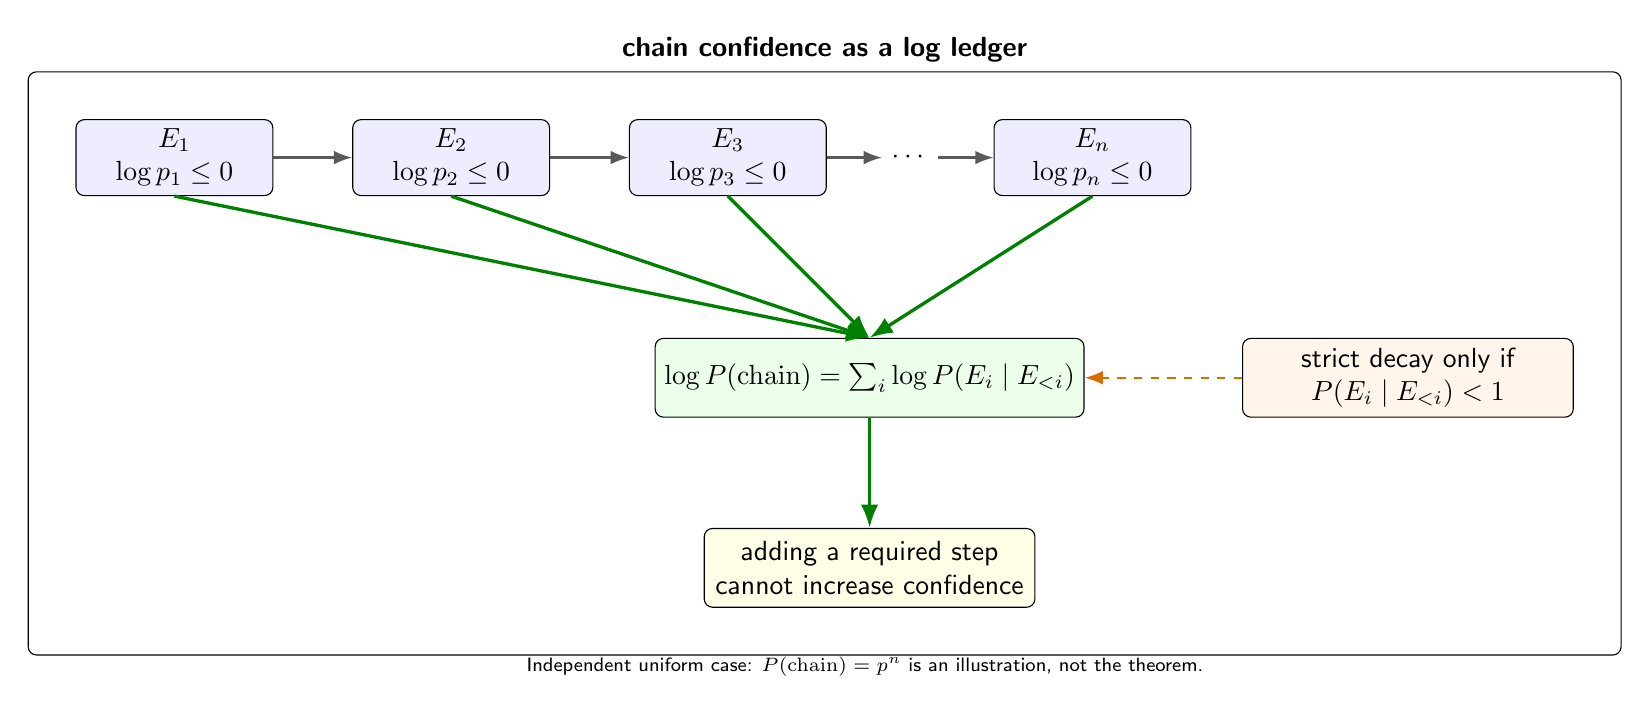
\begin{tikzpicture}[
  font=\sffamily,
  stepbox/.style={draw, rounded corners=3pt, align=center, minimum width=25mm, minimum height=9mm, fill=white},
  sum/.style={draw, rounded corners=3pt, align=center, minimum width=42mm, minimum height=10mm, fill=white},
  arrow/.style={-Latex, thick, draw=black!65},
  good/.style={-Latex, very thick, draw=green!50!black},
  warn/.style={-Latex, thick, dashed, draw=orange!85!black},
  note/.style={align=center, font=\sffamily\scriptsize}
]

\node[stepbox, fill=blue!7] (e1) {$E_1$\\$\log p_1\le 0$};
\node[stepbox, right=10mm of e1, fill=blue!7] (e2) {$E_2$\\$\log p_2\le 0$};
\node[stepbox, right=10mm of e2, fill=blue!7] (e3) {$E_3$\\$\log p_3\le 0$};
\node[right=7mm of e3] (dots) {$\cdots$};
\node[stepbox, right=7mm of dots, fill=blue!7] (en) {$E_n$\\$\log p_n\le 0$};

\draw[arrow] (e1) -- (e2);
\draw[arrow] (e2) -- (e3);
\draw[arrow] (e3) -- (dots);
\draw[arrow] (dots) -- (en);

\node[sum, below=18mm of e3, xshift=18mm, fill=green!8] (ledger)
  {$\log P(\mathrm{chain})=\sum_i\log P(E_i\mid E_{<i})$};
\foreach \x in {e1,e2,e3,en} {
  \draw[good] (\x.south) -- (ledger.north);
}

\node[sum, below=14mm of ledger, fill=yellow!10] (meaning)
  {adding a required step\\cannot increase confidence};
\draw[good] (ledger) -- (meaning);

\node[sum, right=20mm of ledger, fill=orange!8] (strict)
  {strict decay only if\\$P(E_i\mid E_{<i})<1$};
\draw[warn] (strict) -- (ledger);

\node[note, below=5mm of meaning] {
Independent uniform case: $P(\mathrm{chain})=p^n$ is an illustration, not the theorem.
};

\node[draw, rounded corners=3pt, fit=(e1)(e2)(e3)(en)(ledger)(meaning)(strict), inner sep=6mm,
  label={[font=\sffamily\bfseries]above:chain confidence as a log ledger}] {};

\end{tikzpicture}
\end{document}
